\newcommand{\docNome}{ Relazione del Progetto Didattico di Tecnologie Web 2021/2022}
\newcommand{\titoloProgetto}{ Job Finder}
\newcommand{\Tber}{Tommaso Berlaffa } 
\newcommand{\MatT}{1201234}
\newcommand{\Mspa}{Milo Spadotto } 
\newcommand{\MatM}{1122180}
\newcommand{\Plau}{Pietro Lauriola } 
\newcommand{\MatP}{1224820}
\newcommand{\Amat}{Alberto Matterazzo} 
\newcommand{\MatA}{1144597}

\documentclass[11pt, a4paper,table]{article}
\usepackage[utf8]{inputenc}
\usepackage{fancyhdr}
\usepackage{geometry}
\usepackage{xcolor}
\usepackage{array}
\usepackage{graphicx}
\usepackage{hyperref}
\usepackage[document]{ragged2e}
\usepackage[export]{adjustbox}

\definecolor{Blue}{HTML}{004C75}
\definecolor{Yellow}{HTML}{F4E3AE}
\newcolumntype{a}{>{\columncolor{Blue}}c}

\hypersetup{
	pdfborder = {0 0 0}
}
\geometry{a4paper,top=3cm,bottom=3cm,left=2cm,right=2cm}
\title{\textsc{\docNome}}

\date{}
\author{}
\definecolor{footer-gray}{HTML}{808080}
\pagestyle{fancy}
\fancyhf{}
\fancyhead{}

\rhead{\textcolor{footer-gray}{\docNome} }
\lhead{\textcolor{footer-gray}{Job Finder}}
\setlength{\headheight}{14.49998pt}

\fancyfoot{}
\cfoot{\textcolor{footer-gray}{Pagina \thepage } }

\begin{document}
	\maketitle
	\begin{center}
    \begin{figure}[h]
      \includegraphics[scale=0.095]{Images/Logo_Università_Padova.svg.png}
      \hspace{21em}
      
\includegraphics[scale=0.095]{Images/JF_1200.png}
    \end{figure}
    Titolo Progetto : \huge{\titoloProgetto}
		\\
		\vspace{1em}
		\normalsize Email Referente :  \href{mailto:tommaso.berlaffa@studenti.unipd.it}{tommaso.berlaffa@studenti.unipd.it}\\
		
		\vspace{2em}
		\textbf{Componenti del Gruppo :}
		\vspace{0.5em}
		\\ \Tber : \MatT
		\vspace{0.5em}
		\\ \Mspa : \MatM
		\vspace{0.5em}
		\\ \Plau : \MatP
		\vspace{0.5em}
		\\ \Amat : \MatA
    \vspace{0.5em}
    \\ Credenziali :
    \begin{center}
      \begin{tabular}{ |a|c|c| } 
      \hline
      \rowcolor{Blue}
      & \color{Yellow} Nickname & \color{Yellow} Password \\
      \hline
      \color{Yellow} User Generico & user & user\\ 
      \hline
      \color{Yellow} Admin & admin & admin \\ 
      \hline
      \end{tabular}
    \end{center}
    \vspace{0.5em}
    Link al progetto : 

    
	\end{center}

  \newpage
  \tableofcontents
  \raggedright 
	\newpage
	\section{Introduzione}
	\subsection{Abstract}
	Il sito Job Finder si pone come intermediario tra datori di lavori e utenti lavoratori, i quali vogliono sfruttare le proprie competenze per trovare un impiego.\\
  I tipi di lavoro svolti su questo sito sono totalmente di tipo Online. 
	Gli utenti dovranno registrarsi per ottenere diversi privilegi, quali cercare lavoro o creare varie offerte di lavoro, a cui altri utenti potranno rispondere.\\
  Ogni utente loggato avrà inoltre accesso ad un’area riservata, nella quale potrà visualizzare e modificare i propri dati personali e visualizzare uno storico delle proprie offerte e lavori svolti.\\
  Non esiste una divisione tra Utenti Datori di Lavoro e Utenti Lavoratori, esistono solo Utenti normali ed Admin. Questo scelta è stata fatta poiché uno stesso utente si potrebbe trovare a svolgere un lavoro, ma commissionandone un altro allo stesso tempo.\\
  Viene garantita l’accessibilità al sito, rendendo il sito navigabile a chiunque.
  \\
  L’usabilità risulta essere un altro tema di particolare importanza: vengono infatti rispettate le linee guida fornite da W3C e viene fatto in modo che la navigazione sul sito risulti essere il più fluida possibile, fornendo sempre aiuti per fare in modo che l’utente non si senta perso.
	
	
	\newpage
	\section{Analisi}
	
  \subsection{Analisi di Utenza}	
	  Il sito Job finder si rivolge ad un tipo di pubblico esperto, già introdotto al mondo dell’informatica. Viene fatto in modo che anche un utente non esperto e alle prime 
    armi riesca a trovare tutte le informazioni di cui è alla ricerca, senza troppe difficoltà.\\	
    L’utenza di questo sito si quindi può dividere in 3 tipologie:
	  \begin{itemize}
      \item \textbf{Utente nuovo ed inesperto}: arriva sul sito per la prima volta, senza conoscerne alcun dettaglio. Per questo tipo di utente, la pagina di Home deve contenere tutte 
      le informazione necessarie a risolvere qualsiasi dubbio riguardo allo scopo e alle funzionalità del sito. È inoltre necessario fare in modo che questo nuovo utente non si
      senta soverchiato dalle informazioni del sito, per questo motivo viene utilizzato un linguaggio di facile comprensione e vengono mostrare a schermo solamente le 
      informazioni necessarie;
      \item \textbf{Utente in cerca di Lavoro}: utente che conosce il sito e vuole sfruttare le proprie conoscenze ed abilità per ottenere un lavoro. Le zone di ricerca di lavoro e di profilo utente 
      sono quelle dove questo tipo di utente passerà la maggior parte di tempo della navigazione del sito;
      \item \textbf{Utente in cerca di Lavoratori}: utente che conosce il sito e necessita di un lavoratore in grado di svolgere un compito ben specifico. Le zone di creazione lavoro 
      e profilo utente sono quelle dove questo tipo di utente svolgerà la maggior parte delle proprie azioni.
    \end{itemize}
    Il tipo di utente, indipendentemente dal motivo per cui si trova sul sito, viene inoltre diviso in 3 categorie:
    \begin{itemize} 
      \item l’user che non ha ancora fatto il Log In o la Registrazione (\textit{User Non Loggato})
      \item l’user che ha effettuato il Log In (\textit{User Generico}) 
      \item l’utente che ha effettuato il Log In e possiede privilegi (\textit{Amministratore})
    \end{itemize}

  \subsection{Casi d'Uso}
    Alle 3 tipologie di utenza precedente elencate saranno accessibili diverse pagine:
    \begin{itemize}
      \item a tutti gli utenti saranno visibili le pagine Home, FindJob, Login, SignUp e FAQ;
      \item a tutti gli utenti che hanno effettuato il login saranno visibili tutte le pagine (comprendono CreateJob, UserProfile e ViewJob/ViewUser);
      \item agli utenti Amministratori saranno visualizzabili ulteriori elementi nelle pagine che permettono modifiche a dati/informazioni di altri utenti, in aggiunta ad una pagina per cercare specifici utenti e lavori.
    \end{itemize}

  \subsection{Analisi Requisiti} 
    Il sito si occupa principalmente di soddisfare 2 richieste:
    \begin{itemize}
      \item \textbf{Ricerca di un lavoro}, tramite le pagine di visualizzazione dei lavori disponibili, a cui un utente interessato può fare una proposta;
      \item \textbf{Ricerca di un lavoratore}, tramite la creazione di un’offerta di lavoro, al quale il possibile candidato potrà proporsi.
    \end{itemize}
    Oltre a questi due requisiti, su cui si basa l’intero sito, sono presenti altre funzionalità di interesse, quali :
    \begin{itemize}
      \item Descrizione delle funzionalità del sito;
      \item Sign Up, Log In, Log Out. La visualizzazione di alcune pagine, come lo User Profile o la Creazione di una Offerta di Lavoro, non sono visibili agli utenti non 
      attualmente loggati;
      \item Cronologia dei Lavori Svolti (sia da parte del creatore dell’Offerta, sia da parte del Lavoratore), Cronologia delle Offerte e Offerte attualmente in atto;
      \item Possibilità di filtrare le varie offerte di Lavoro;
      \item Possibilità di Visualizzare informazioni su Utenti che si propongono per un offerta di lavoro:
      \item Lettura e Scrittura di Feedback sul Lavoro svolto.
    \end{itemize}

	\section{Progettazione}
	
  \subsection{Design}
  Per il design del sito, sono state perseguite due principali strade:
  \begin{itemize}
    \item \textit{Desktop First}: il nostro sito si rivolge ad un utenza molto tecnica e pensiamo che l'utilizzo del sito avverrà principalmente da Desktop. Viene comunque data importanza all'utenza che deciderà di approcciarsi a questo sito tramite smartphone.
    \item \textit{Layout a 4 Pannelli}: utilizzato in tutte le pagine del sito tranne UserProfile, dove viene utilizzato un Layout a 5 Pannelli, aggiungendo una \textbf{Sidebar} per la navigazione tra le sottopagine di User Profile.
  \end{itemize}

  I 4 pannelli che compongono il layout delle nostre pagine sono:
  \begin{enumerate}
    \item \textbf{Header}: composto dal logo del sito e dai link alle altre pagine;
    \item \textbf{Breadcrumb}: contiene i Link alle pagine "precedenti" a quella che si sta attualmente visitando; il breadcrumb è di vitale importanza per far sì che l'utente
      non si senta perso nella navigazione del sito. Nel caso del nostro sito, il breadcrump è stato scritto in maniera da simulare un path di un filesystem;
    \item \textbf{Main}: corrisponde al vero e proprio contenuto della pagina;
    \item \textbf{Footer}: contiene informazione su come contattare l'Admin in caso di problemi e il link per le FAQ.
  \end{enumerate}
  
  Il quinto pannello, overro la \textbf{sidebar}, è utilizzato nella pagina UserProfile. 
  Questa pagina raccoglie informazioni utili dell'utente $($informazione su utente, sui lavori svolti e proposti$)$, la possibilità di modificare i propri dati utente ed è accessibile solo dallo stesso utente.


  \subsection{Database}
  Il database risulta essere una parte cruciale del nostro sito, poiché la funzione stessa del sito è gestita su quest'ultimo.
  \begin{figure}[h]
    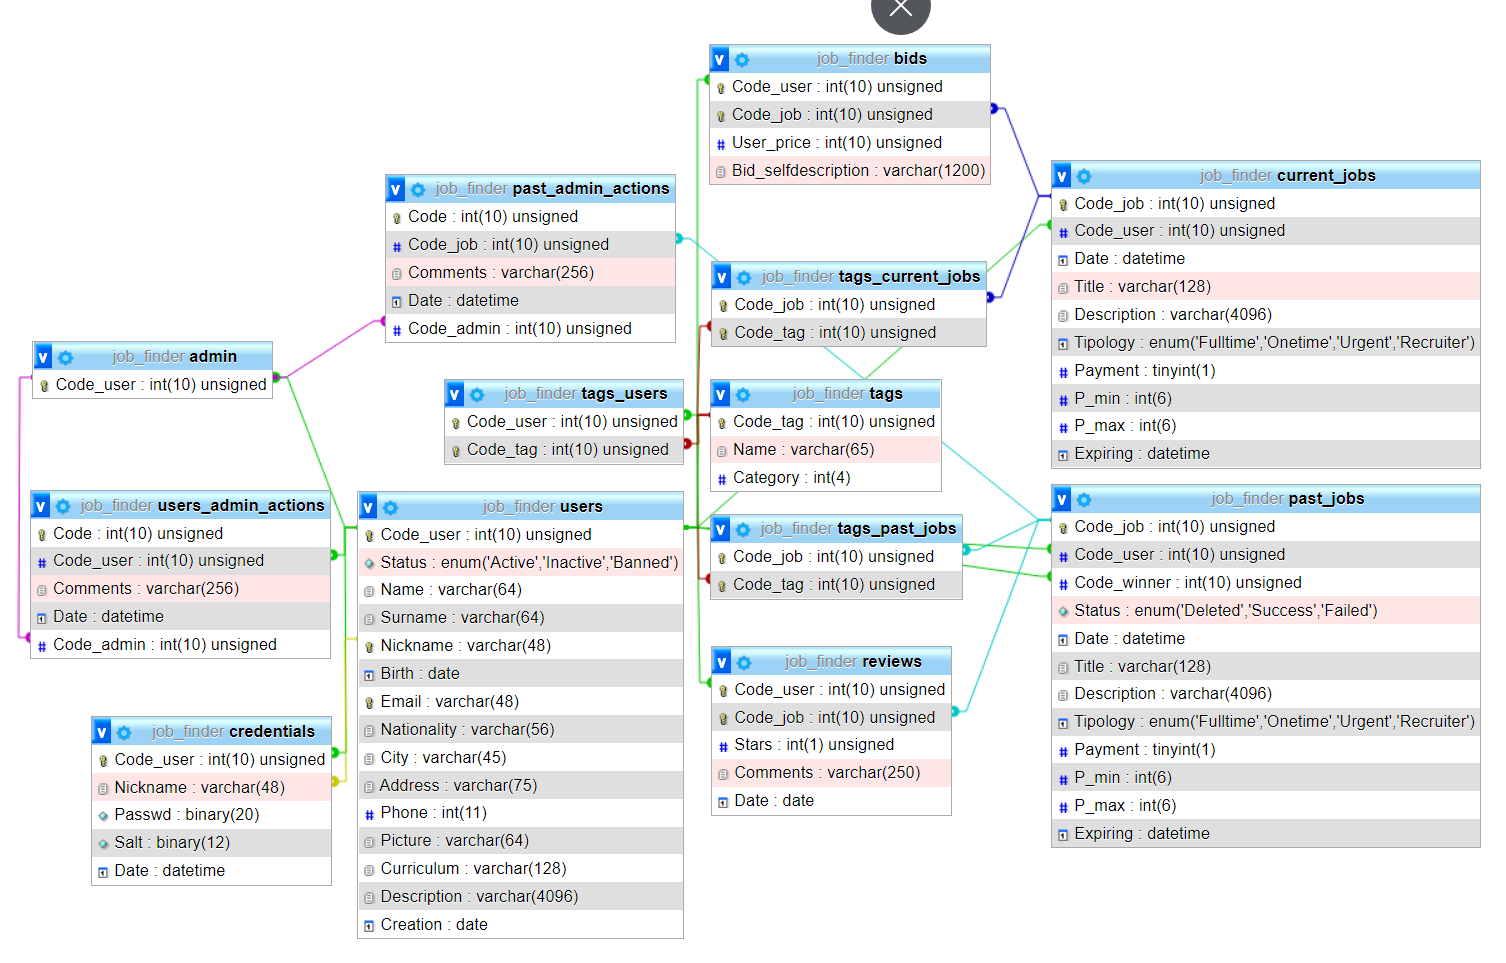
\includegraphics[scale=0.5]{Images/DB2.png}
    \caption{Schema del database}
    \centering
  \end{figure}
  Le tabelle che compongono il nostro sono :
  \begin{itemize}
    \item \textbf{users e credentials} : users contiene i dati utente e Credentials contiene le credenziali, questi dati sono divisi in due tabelle per evitare leak di informazioni;
    \item \textbf{current\textunderscore jobs e bids} : current\textunderscore job contiene i dati inerenti alle offerte di lavoro, bids contiene i dati inerenti alle candidature per le offerte in questione;
    \item \textbf{past\textunderscore jobs e reviews} : past\textunderscore jobs contiene i dati inerenti alle offerte di lavoro eliminate, fallite o avvenute con successo; reviews contiene i feedback delle past\textunderscore jobs avvenute con successo;
    \item \textbf{tags, tags\textunderscore users, tags\textunderscore past\textunderscore jobs, tags\textunderscore current\textunderscore jobs} : tags contiene tutti i possibili tag presenti nel sito, tags\textunderscore users, tags\textunderscore past\textunderscore jobs e tags\textunderscore current\textunderscore jobs contengono le chiavi delle rispettive tabelle e di tags per associare le due tabelle;
    \item \textbf{admin, user\textunderscore admin\textunderscore actions e past\textunderscore admin\textunderscore actions} : admin contiene i code\textunderscore user degli utenti admin, le tabelle user\textunderscore admin\textunderscore actions e past\textunderscore admin\textunderscore actions contengono rispettivamente gli storici delle azioni eseguite dagli admin su utenti e su offerte di lavoro. 
  
  \end{itemize}

  Viene utilizzato PHP per interrogare il database, tramite una classe specializzata chiamata DBAccess.php. \\
  Molte pagine all'interno del nostro sito vengono riempite dinamicamente con i risultati forniti dal database, 
  alcuni esempi possono essere la ricerca dei lavori su findJob, la quale utilizza sia PHP che AJAX, o le visualizzazione dei dati degli utenti di ViewUser.

  

  \subsection{Obiettivi}
  Il gruppo si è prefissato alcuni obiettivi da perseguire durante la realizzazione di questo progetto, al fine di mantenere l'accessibilità e l'usabilità come priorità e migliorare il più possibile l'esperienza utente :
  \begin{itemize}
    \item utilizzo di tag \textit{alt} per tutte le immagini presenti nel sito. Questo non è utile solamente quando l'immagine non è disponibile, ma inoltre risulta essere fondamentale poiché è cio che viene letto dagli screen reader, quindi elemento necessario se si vuole fornire la possibilità ad un utente che utilizza questo strumento di comprendere il contesto o il significato di un'immagine.
        Esistono alcuni casi in cui \textit{alt} viene inserito con valore vuoto, questo per due motivi :
    \begin{itemize}
      \item l'immagine è associata ad un link, come nel caso dei link dell'header. In questo caso, aggiungere un tag che ripeta il significato del link viene considerata bad practise poiché l'utente che utilizza screen reader dovrà ascoltare due volte lo stesso elemento e l'utente che si ritrova con l'immagine non disponibile si troverà con una scritta "raddoppiata", creando confusione;
      \item l'immagine è di contesto, non ha un significato specifico o importanza a livello di contenuto; viene quindi tenuto alt vuoto.
    \end{itemize}
    \item reinserimento automatico degli input inseriti dall'utente quando avviene il reindirizzamento della pagina sulla stessa 
     $($es: il submit della form di createJob richiama createJob.php che, controllato i dati e confermando un possibile errore, rimanda alla pagina createJob ma ricaricando i valori correttamente inseriti $)$;
    \item uso intelligente del \textit{breadcrumb}, poiché il breadcrumb fornisce informazione all'utente su come é arrivato su quella parte del sito, è fondamentale che il breadrcumb risulti completo;
    \item meccanismi di \textit{hidden help} e \textit{gobacktothetop}, entrambi meccanismi che utilizzano $<$a href="\#"$>$ per condurre l'utente su diversi elementi della pagina. I primi vengono utilizzati da utenti che utilizzano screen reader, i secondi vengono utilizzati quando le pagine risultano verticalmente troppo grandi per tornare all'inizio della pagina;
    \item aiuti utente e indicazione sulla correzioni di errori nell'inserimento dati. Nel caso in cui avvengano degli errori, quali mancanza di input o altre tipologie di errori, verranno riportati i cambiamenti da attuare ed il motivo dell'errore, in modo da aiutare l'utente a inserire i dati correttamente.
  \end{itemize} 
  \newpage
	\section{Presentazione}

  \subsection{Presentazione Generale}
    Per il nostro sito è stato scelto come colore principale il blu. Abbiamo scelto questo colore perché spesso viene associato a sensazioni di stabilità e affidabilità, che il nostro sito vuole trasmettere. 
    Questo è il pattern di colori utilizzati per il tema del sito:
    \begin{figure}[h]
      
\includegraphics[scale=0.8]{Images/Palette1.png}
      \caption{Palette Colori Utilizzata per il sito}
      \centering
    \end{figure}

  \subsection{Desktop}
    Come dimensione massima per la versione desktop si è deciso di utilizzare 1200px, al fine di evitare difficoltà da parte dell'utente a visualizzare la pagina nella sua interezza. \\
    È presente un punto di rottura a 959px, al fine di migliorare la visibilità e le dimensioni di alcuni elementi.

  \subsection{Mobile}
    In modo simile alla versione Desktop, per la visualizzazione lato Mobile si è optato un punto di rottura di 694px; questo permette di gestire al meglio la visualizzazione della pagina su dispositivi mobile. \\
    La visualizzazione Mobile differisce principalmente per alcuni elementi, quali:
    \begin{itemize}
      \item il footer viene rimpiazzato con l'header e viceversa. In questo modo, sarà più semplice per l'utente da mobile utilizzare i link dell'header che potranno essere utilizzati come bottoni di un app;
      \item il logo viene rimosso;
      \item i contenuti che precedentemente venivano visualizzati di lato o in parallelo vengono visualizzati in verticale per migliorare l'esperienza utente;
    \end{itemize}
    Inoltre, per la pagina di User Profile, viene utilizzata una checkbox nascosta, selezionabile tramite una label, che mostra e nasconde la barra laterale. Questa scelta è stata fatta poiché una barra
    laterale fissa su dispositivi mobile avrebbe occupato troppo spazio.
  
  \subsection{Print}
    Per la funzionalità di stampa si è deciso di andare ad eliminare Header, sidebar e Footer. \\
    Il breadcrumb viene riadattato e vengono tolti alcuni elementi come :
    \begin{itemize}
      \item le form;
      \item i link che portano ad altre parti della pagina;
    \end{itemize}
    Gli elementi che verranno quindi visualizzati saranno il testo scritto dentro al main, le tabelle e i div che contengono informazioni. \\
    Generalmente non verranno visualizzate le form, tranne nelle pagine in cui sono presenti solamente quelle.
	\section{Implementazione}
	

  \subsection{HTML}
  Per questo progetto è stato deciso di utilizzare HTML5 per gestire la struttura. \\
  In ogni pagina HTML saranno presenti i tag meta, che andranno ad indicare diverse informazioni come:
  \begin{itemize}
    \item autori del file;
    \item titolo e descrizione della pagina;
    \item keyword utilizzate per la ricerca della pagina sul web.
  \end{itemize}
  Nel nostro caso, le parole utilizzate come keyword sono il titolo del sito e delle parole che hanno a che fare con lo scopo della pagina, come nel caso di findJob in cui le parole utilizzate saranno "Find a Job Offer".
  I file HTML si andranno a dividere in 2 categorie :
  \begin{itemize}
    \item Pagine HTML, che vengono caricate da PHP e a cui vengono modificati alcuni valori;
    \item Elementi HTML, ovvero file HTML che contengono solo alcuni elementi che poi verranno modificati da PHP e caricati sull'effettiva pagina HTML;
  \end{itemize}

  
  \subsection{CSS}
  Per la parte di presentazione, sono presenti 3 file:
  \begin{itemize}
    \item style.css: per i dispositivi desktop;
    \item mobile.css: per i dispositivi mobile;
    \item print.css: per le funzioni di stampa.
  \end{itemize}
  Viene garantita la separazione tra struttura e presentazione. Per questo motivo non vengono dichiarati tag style nei file html e si utilizzano file esterni piuttosto che css inline o embeded.
  Per la definizione di dimensioni all'intero del sito, si è optato nella maggior parte dei casi per unità misura gli em o percentuale. Alcuni elementi invece, come le icone, utilizzano px.\\
  Viene fatto largo uso di display flex per allieare elementi orizzontalmente o verticalmente in modo da migliorare l'inpaginazione di elementi su diverse tipologie di schermi. \\
  Vengono inoltre utilizzati display grid per diversi elementi, come le form di cambio dati utente e le informazioni relative all'offerta di lavoro su FindJob.
  
  \subsection{JavaScript}
  Javascript è uno dei linguaggio utilizzati per il comportamento ed è stato utilizzato per 3 funzionalità:
  \begin{itemize}
    \item controlli su form, per fare in modo che la pagina non dovesse venire ricaricata nel caso ci fossero errori facilmente risolvibili. Alcuni esempi sono il controllo della password, per confermare se soddisfa i requisiti minimi di complessità;
    \item filtraggio tramite tag per findjob e ricerca ed inserimento tag per createJob e area privata;
    \item ricerca tramite input testuale per la zona riservata agli admin.
  \end{itemize}
  
  Viene inoltre fatto utilizzo di \textbf{AJAX} per ottenere i tag dal server senza dover aggiornare la pagina.

  \subsection{PHP}
  Ogni pagina nel nostro sito viene caricata tramite pagina PHP, questo perché alcuni elementi presenti nell'header verranno visualizzati in maniera diversa in base allo stato di login del'utente. \\
  I file PHP saranno quindi di 3 tipologie:
  \begin{itemize}
    \item file PHP che caricano le pagine HTML e modificheranno alcuni valori, mantenendo così la divisione tra comporamento e struttura poiché quest'ultima sarà descritta nel file .html;
    \item file PHP DBAccess.php, utilizzato per l'interazione con il database;
    \item file PHP che effettuano azione alla fine delle quali reindirizzano ad un'altra pagina.
  \end{itemize}

  Vengono eseguiti controlli sull'input, quali:
  \begin{itemize}
    \item filter\textunderscore var, data una variabile ed il tipo di filter effettua delle operazioni per ottenere una stringa filtrata;
    \item trim, rimuove spazi vuoti all'inizio e alla fine di una stringa.
  \end{itemize}

  \subsection{MySql}
  Per la gestione ed il mantenimento dei dati si é scelto di utilizzare MySql. Viene utilizzata l'estensione misqli per tutte le funzioni che usano MySql. \\
  Si utilizza bind\textunderscore parameters per evitare query injection.
  \section{Sito Web}
	Il sito sarà quindi diviso nelle seguenti pagine :
  \begin{itemize}
    \item \textbf{Homepage} : pagina centrale del sito, mostra delle informazioni generiche con lo scopo di aiutare chi arriva per la prima volta su questa pagina;
    viene utilizzato un layout grid per posizionare gli elementi in maniera corretta nella schermata; sono presenti due immagini, di puro abbellimento, quindi con alt vuoto;
    nella versione mobile, il layout grid viene modificato per semplificare la navigazione tramite scorrimento, cambiando gli elementi affiancati e ponendoli verticalmente su tutta la schermata;
    \item \textbf{FAQ} : pagina composta prevalentemente da testo, con domande e risposte frequenti; seguente l'ordine degli header, ovvero h1 seguito da h2, modificati con css per rispettare lo stile che volevamo utilizzare ma mantendendo la correttezza del significato dell'elemento;
    \item \textbf{Login} : pagina contentente 1 form con 2 campi, username e password; la password non viene visualizzata e verrà utilizzato un "salt" per effettuare la codifica; nel caso l'inserimento non avvenga correttamente, viene visualizzato un messaggio d'errore che punta ad \#user;
    \item \textbf{Sign Up} : pagina contentente 1 form, divisa in 4 fieldset, utilizzata per la registrazione al sito;
    la registrazione richiederà diversi passaggi e potrebbe risultare lunga e faticosa, abbiamo quindi deciso di dividere la form in 4 fieldset, visualizzando 1 fieldset
    per volta, in modo tale da controllare i campi ad ogni cambio di fieldset, evitando così errori dovuti al non corretto inserimento di dati nella form; in questo modo se un username è già in uso o se la password è non valida, questa verrà notificato nel primo fieldset e non dopo aver completato tutta la form;
    \item \textbf{FindJob} : pagina centrale per lo scopo del nostro sito, utilizza un layout flex diviso tra form di filtering e lista dei lavori, divisi tramite paginazione;
    per l'inserimento dei tag, si è discusso molto su quale elemento utilizzare ed il gruppo è arrivato alla conclusione che elementi come select con attributo multiple o datalist non facessero al nostro caso;
    abbiamo quindi deciso di utilizzare un input che in base ai risultati ottenuti tramite AJAX crea dei bottoni che rappresentano i tag, questi possono essere aggiunti/tolti e verranno utilizzati nel filtering;
    sono stati predisposti degli hiddenHelp per aiutare utenti che utilizzano screen reader ad utilizzare al meglio questo meccanismo;
    \item \textbf{CreateJob} : pagina utilizzata per la creazione di un annuncio, contiene una form da riempire con tutti i dati necessari;
    \item \textbf{UserProfile} : zona riservata di ogni utente che ha effettuato il login al sito; divisa in 6 sottopagine :
    \begin{enumerate}
      \item \textit{Welcome} : visibile quando si entra per la prima volta dopo il login nel sito;
      \item \textit{User Info} : mostra le informazioni dell'utente e le ultime 3 reviews;
      \item \textit{Your Job Offer} : pagina contentente 2 tabelle, la prima contentente le offerte create dall'utente che sono in corso o aspettano la scelta di un vincitore; la seconda contente i lavori passati creati sempre dall'utente;
      \item \textit{Your Bids} : pagina specchiata rispetto a "Your Job Offer", contiene 2 tabelle simili ma riguardo alle Bids presenti e passate;
      \item \textit{User Settings} : contiene 2 form, una per la modifica dei dati utente, caricata tramite PHP con i dati utente; la seconda per la modifica dei tag, caricata con i tag utente;
      \item \textit{Change Password} : contiene una form per il cambio della password;
    \end{enumerate}
    \item \textbf{Viste} : nel sito sono presenti 2 pagine "viste", ovvero ViewJob e ViewUser.
    \begin{itemize}
      \item \textit{ViewUser} : vista sulle informazioni dell'utente. Solo alcune informazioni vengono mostrate, per mantenere la privacy; vengono inoltre mostrate le ultime 5 review, ma senza descrizione;
      \item \textit{ViewJob} : vista sulle informazioni di un lavoro. Un lavoro può essere Past o Current e può appartenere a diversi status :
      \begin{itemize}
        \item Se il lavoro è current ed il tempo non è terminato, un utente potrà effettuare una bid; a sua volta il creatore della offer potrà eliminare o terminare il lavoro;
        \item Se il lavoro è current ma il tempo è terminato, non si potranno effettuare bid; il creatore della offer potrà eliminare il lavoro o decidere chi sarà il vincitore nel caso in cui ci siano bid;
        \item Se il lavoro è past e c'è un vincitore, il creatore della offer potrà effettuare una review sull'utente che ha effettuato il lavoro;
        \item Se il lavoro è past e non ci sono stati vincitore, non saranno possibili altre azioni.
      \end{itemize}
    \end{itemize}
    \item \textbf{Admin} : le pagine di admin saranno visibili su UserProfile \/ Welcome e UserProfile \/ UserInfo. Queste saranno 4 e conterranno rispettivamente :
    \begin{enumerate}
      \item \textit{Admin History} : contiene 2 tabelle con le azioni compiute dagli admin;
      \item \textit{Admin Users} : contiene lista degli user con possibilità di ricerca per nome; ogni nome avrà un link che invia alla pagina ViewUser, dove l'admin potrà bannare o "sbannare" un utente;
      \item \textit{Admin Offers} : contiene lista delle offerte con possiblità di ricerca per titolo; l'Admin potrà cancellare l'offerta, rendendola un past job con status "Deleted";
      \item \textit{Admin Jobs} : contiene lista dei lavori con possibilità di ricerca per titolo, l'Admin potrà eliminare l'offerta, cambiando status ad un past job e rendendolo "Deleted".
    \end{enumerate}
  \end{itemize}
  \section{Test}

  Gli strumenti utilizzati per il Testing generale del sito sono stati:
  \begin{itemize}
    \item \textit{WAVE}, ovvero uno strumento utile a rendere il proprio sito più accessibile ad utenti con disabilità. Questo strumento infatti può identificare diversi errori di accessbilità (come quelli presenti nelle Guideline di WCAG). I test di WAVE sono stati fatti tramite estensioni del browser Chrome.
    \item \textit{Silktide}, un'estensione web che permette di testare la propria pagina andando a simulare diverse disabilità, tra cui (per citarne alcune) dislessia e daltonismo. Questo tipo di software ci permette quindi di rendere le nostre pagine più facilmente esplorabili da questa tipologie di utenza.
  \end{itemize}
  Sono stati inoltre utilizzati strumenti più specifici per altri tipi di testing.
	
  \subsection{Testing di Compatibilità}
    Il testing delle pagine è stato effettuato su diversi browsers, ovvero :
    \begin{itemize}
      \item Google Chrome, su cui è stato testato principalmente il sito;
      \item Mozilla Firefox;
      \item  Microsoft Edge;
      \item Safari.
    \end{itemize}
    Abbiamo deciso di tralasciare Internet Explorer poiché quest'ultimo risulta non essere più supportato.

  \subsection{Testing del contrasto dei Colori} 
    WAVE permette, in maniera molto semplice, di controllare se nel sito sono presenti contrasti a livello cromatico che potrebbero risultare fastidiosi ad alcune categorie di utenti.
    Inoltre, è stato anche utilizzato il \href{https://webaim.org/resources/contrastchecker/}{Contrast Checker} fornito da WebAim per assicurarci che i colori da noi scelti risultassero non fastidiosi all'utente.

  \subsection{Testing di Grandezza delle Pagine}
    Una caratteristica molto importante di un buon sito web è la leggerezza, infatti nella creazione di un sito web è buona pratica fare in modo che le pagine non risultino essere troppo pesanti. Questo potrebbe rendere il rendering delle pagine lento e creare una sensazione negativa nell'utente.\\
    Per questo motivo, viene consigliato di fare in modo che il preso delle pagine sia il minore possibile, generalmente mantenendolo tra i 2 ed 1 Megabyte. 

  \subsection{Testing di Altezza delle Pagine}
    Vengono disposte pratiche per fare in modo che non vi siano pagine "troppo alte" e, in caso questo succeda comunque, vengono predisposti meccanismi per tornare indietro. \\
    Esempi di questi meccanismi possono essere :
    \begin{enumerate}
      \item Nella pagina \textit{Findjob}, i lavori posso idealmente essere migliaia ma ne verranno solamente visualizzati un massimo di 10 per volta. Questo avviene grazie alla divisione del contenuto in sottopagine;
      \item Nelle pagine \textit{UserProfile} di \textit{Your Job Offers} e \textit{Your Bids}, le tabelle vengono riempite dinamicamente con i dati presenti nel database. Per questo motivo, non conoscendo la Grandezza
      delle tabelle, vengono creati dei link di "go back to the top" per far sì che, nel caso la tabella generata risulti essere troppo grande, l'utente abbia comunque la capacità di tornare all'inizio della pagina senza alcuna difficoltà.
    \end{enumerate}
	\section{Validazione}
La validazione risulta essere uno dei punti cruciali del progetto. Questo perché permette di verificare che siano stati rispettati gli standard W3C per quanto riguarda HTML e CSS, permettendo così di avere del codice corretto.\\
Codice corretto e validato conferma la solidità di un sito web sui diversi browser. \\
Per validare il sito sono stati utilizzati i seguenti strumenti:
\begin{itemize}
	\item \textbf{W3C HTML Validator}: è un tool online che, dato in input un file .html o del codice HTML, effettua la validazione del codice HTML al fine di assicurare la qualità della pagina.
	\item \textbf{W3C CSS Validator}: è un tool online che, dato in input un file .css o del codice CSS, effettua la validazione del codice CSS, permettendo così di assicurare la validità del codice sottoposto.
\end{itemize}
  \section{Suddivisione del Lavoro}
Tutti i membri del gruppo hanno lavorato alla creazione del progetto. La codifica nei linguaggi HTML e PHP è stata eseguita da ogni membro del gruppo e la stesura iniziale 
dei punti cardine del progetto è stata fatta in gruppo. \\
Di seguito sono elencati i ruoli
\begin{itemize}
	\item \textbf{Tommaso Berlaffa}
	\begin{itemize}
    \item Pagina UserProfile
    \item Stesura relazione
	\end{itemize}
	\item \textbf{Pietro Lauriola}
	\begin{itemize}
    \item Pagina CreateJob
		\item Test di accessibilità
		\item Test di usabilità
	\end{itemize}
	\item \textbf{Milo Spadotto}
	\begin{itemize}
    \item Pagine Login e SignUp
		\item Sviluppo DB
	\end{itemize}
	\item \textbf{Alberto Materazzo}
	\begin{itemize}
    \item Pagina FindJob
		\item Test di accessibilità
		\item Test di usabilità
	\end{itemize}
\end{itemize}

\end{document}